\documentclass[11pt]{article}

\usepackage[final]{acl}

\usepackage{times}
\usepackage{latexsym}

\usepackage[T1]{fontenc}

\usepackage[utf8]{inputenc}

\usepackage{microtype}

\usepackage{inconsolata}

\usepackage{graphicx}
\graphicspath{{../graphs/}}

\title{Word-in-Context Classification for Human-Machine Mixed Text Detection}

\author{
    Anya Kiewit \\ Address line \\ Address line \\ \And
    Isabelle \\ Address line \\ Address line \\ \And
    Johan Wols \\ Address line \\ Address line \\ \And
    Marten de Jong \\ 4557182 \\  marten.de.jong.4@student.rug.nl 
}

\begin{document}
\maketitle
\begin{abstract}

\end{abstract}

\section{Introduction}

\section{Related Work}

\textcolor{red}{Maybe, Maybe not}

\paragraph{SemEval-2024 Task 8 and Subtask C}
Our research is within in the framework of SemEval-2024 Task8, which benchmarks Multigenerator, Multidomain and Multilingual Machine-Generated Text Detection.
Subtask C presents the challenge of boundary detection in mixed texts. The objective is to identify the word index where a document transitions from human-written to machine-generated content.
Evaluating this requires models to identify abrupt shifts in stylistic consistency and token predictability.

\paragraph{Stylometry and Probabilistic AI Text Detection}
Historically authorship attribution and text classification relied heavily on stylometric features to establish an author's unique fingerprint \cite{neal2017surveying}.
Surface-level markers such as average word length, punctuation frequency and capitalization patterns have proven to be robust discriminators of human writing styles \cite{neal2017surveying}.

However with the rise of Large Language Models (LLMs), detection mechanisms have increasingly adopted probabilistic approaches.
Masked Language Models (MLMs)ct predictive features such as token log-probability, rank and perplexity.
Recently, Xu and Sheng (2024) demonstrated the robustness of this approach by utilizing MLM-based perplexity to successfully detect AI-generated sequences \cite{xu2024detecting}.
Their findings emphasize that AI-generated text, in their case code, consistently exhibits lower and more uniform perplexity compared to the natural variance of human authorship \cite{xu2024detecting}.
% This validates our use of both stylometric baseline features and MLM-derived metrics to identify the exact boundary where text shifts from human variance to machine predictability.

\section{Data}

\subsection{Dataset Description}

\textcolor{red}{Written texts where each token separated by space is either labeled with 0 for Human written or Machine written text}
\\ \\
\textcolor{red}{Statistics of the data}

The data for this study is provided by the SemEval-2024 Task 8 organizers for Subtask C (Human-Machine Mixed Text Detection).
The dataset consists of documents where the first part is written by a human and the following part is generated by a LLM.
The data is structured in JSON Lines (JSONL) format, where each entry contains a unique id, the raw text, and a list of labels.
The label represents whether the token at the 0-based index is human-written (0) or machine-written (1).



\section{Method}

\subsection{Task Formulation}

\textcolor{red}{small summary of the task, what we are trying to predict}

\subsection{Preprocessing}

\textcolor{red}{Split only on (" "), lemmatization/stemming and punctuation handling kept to a minimum}

\subsection{Feature Engineering}

\textcolor{red}{Summary of the kinds of features where trying to get and what will eventually go into the models}

\subsubsection{Positional Features}

\textcolor{red}{absolute doc pos and relative doc pos}

\subsubsection{Statistical Features}

\textcolor{red}{Describe the retrieved features}

\subsubsection{MLM Features}

\textcolor{red}{Describe what model used and why. What the effect of this is and how the results are to be interpreted}

\subsection{Models}

\textcolor{red}{Why we've chosen the models we chose}

\subsubsection{Naive Bayes}

\textcolor{red}{Describe Naive Bayes, and describe the baseline}

\subsubsection{Logistic Regression}

\textcolor{red}{Describe the model and the feature retrieval}

\subsubsection{SVM}

\textcolor{red}{Describe the experiments}

\subsubsection{Random Forest}

\textcolor{red}{TODO}

\section{Experiments}

\textcolor{blue}{Don't know about this yet. Maybe explicitly state why we've not chosen to do anything significant with this}

\section{Results}

\begin{figure}[t]
    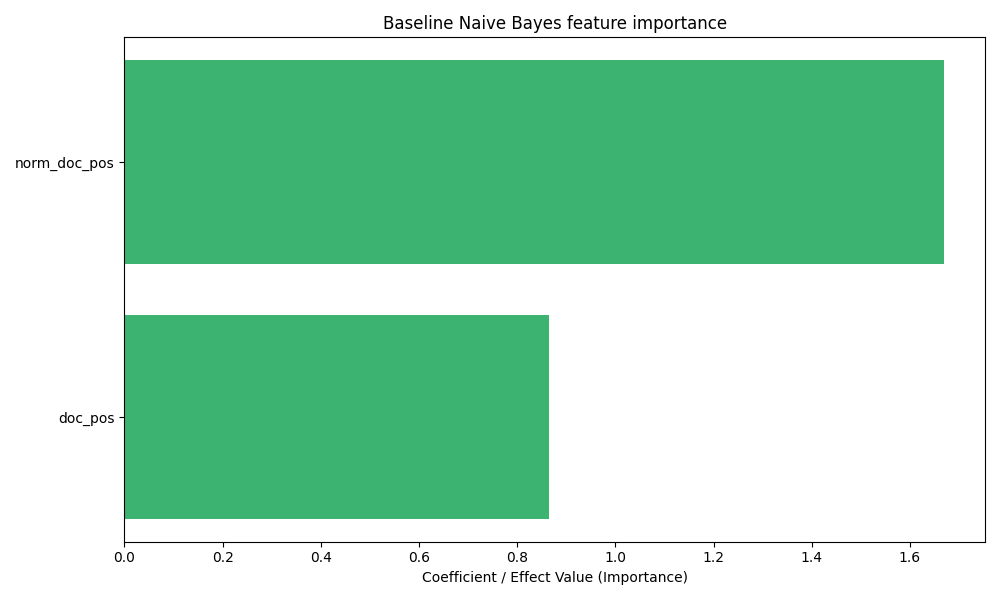
\includegraphics[width=\columnwidth]{baseline_naive_bayes_feature_importance_importance.png}
    \caption{Feature importances for the baseline Naive Bayes model.}
\end{figure}

\textcolor{red}{TODO}

\section{Conclusion}

\textcolor{red}{TODO}

\section{Limitations}

\textcolor{red}{TODO}

\section{Future Work}

\textcolor{red}{Try different context window sizes. Try different models, transformer based sequence tagging}

\bibliography{custom}

\newpage

\appendix

\section{Individual Contributions}

\subsection{Anya Kiewit}

\subsection{Isabelle}

\subsection{Johan Wols}

\subsection{Marten de Jong}

\begin{itemize}
    \item Project Setup/Management
          \begin{itemize}
              \item Trello
              \item Python Project
              \item Small bugfixes if occurred after merging
              \item File-handling
          \end{itemize}
    \item Preprocessing
          \begin{itemize}
              \item Train-Val split
              \item Context Windows
          \end{itemize}
    \item Feature Engineering
          \begin{itemize}
              \item MLM-features
          \end{itemize}
    \item Evaluation
          \begin{itemize}
              \item MAE
              \item Visualization
          \end{itemize}
    \item Models
          \begin{itemize}
              \item SVM
          \end{itemize}
    \item Report
          \begin{itemize}
              \item
          \end{itemize}
\end{itemize}

\end{document}